\subsection{Vector Fields}

\begin{example}[Intuition]
  A \emph{fluid flow velocity field} assigns each position a velocity vector:
  \[
    f(\text{position}\in\R^2) = \text{velocity}\in\R^2
  \]

  \begin{center}
    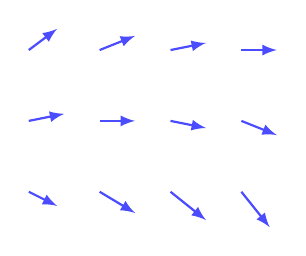
\begin{tikzpicture}[scale=0.9, >=latex]
			\foreach \x/\y/\dx/\dy in {
					-1.5/1/0.4/0.3, -0.5/1/0.5/0.2, 0.5/1/0.5/0.1, 1.5/1/0.5/0,
					-1.5/0/0.5/0.1, -0.5/0/0.5/0, 0.5/0/0.5/-0.1, 1.5/0/0.5/-0.2,
					-1.5/-1/0.4/-0.2, -0.5/-1/0.5/-0.3, 0.5/-1/0.5/-0.4, 1.5/-1/0.4/-0.5
				} {
					\draw[->, thick, blue!70] (\x,\y) -- ++(\dx,\dy);
				}
		\end{tikzpicture}
  \end{center}
\end{example}

\begin{definition}{Vector Field}{vector-field}
  Let $D\subseteq\R^n$. A \emph{vector field} on $D$ is a function $\mathbf{F}$
  that assigns each point $\mathbf{x}\in D$ an $n$-dimensional vector $\mathbf{F}(\mathbf{x})$:
  \[
    \mathbf{F}\colon D\subseteq\R^n\to\R^n
  \]
  The cases $n=2$ and $n=3$ are most common.
\end{definition}

\begin{example}[Vortex]
  Sketch $\mathbf{F}(x,y) = \ve{-y,\,x}$. Samples:
  \[
    \mathbf{F}(1,0) = \ve{0,1},\quad
    \mathbf{F}(2,0) = \ve{0,2},\quad
    \mathbf{F}(0,1) = \ve{-1,0},\quad
    \mathbf{F}(-1,1) = \ve{-1,-1}
  \]

  \begin{center}
    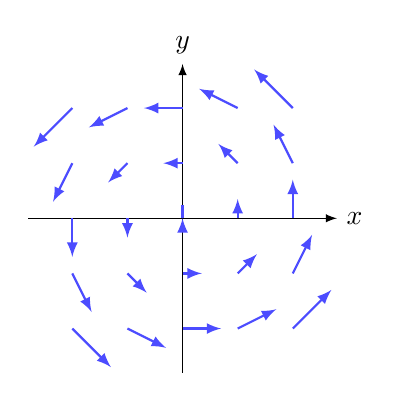
\begin{tikzpicture}[scale=0.7, >=latex]
			\draw[->] (-2.8,0) -- (2.8,0) node[right]{$x$};
			\draw[->] (0,-2.8) -- (0,2.8) node[above]{$y$};
			\foreach \x in {-2,-1,0,1,2} {
					\foreach \y in {-2,-1,0,1,2} {
							\pgfmathsetmacro{\dx}{-\y*0.35}
							\pgfmathsetmacro{\dy}{\x*0.35}
							\draw[->, thick, blue!70] (\x,\y) -- ++(\dx,\dy);
						}
				}
		\end{tikzpicture}
  \end{center}
\end{example}

\begin{example}[Gravity]
  Place mass $M$ at the origin. The gravitational force on a mass $m$ at position $\mathbf{x}$ is
  \[
    \mathbf{F}(\mathbf{x}) = -\frac{GMm}{\lVert\mathbf{x}\rVert^2}\,\hat{\mathbf{x}},
    \qquad \hat{\mathbf{x}} = \frac{\mathbf{x}}{\lVert\mathbf{x}\rVert}
  \]

  \begin{center}
    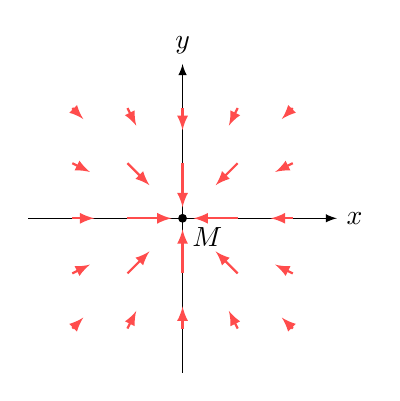
\begin{tikzpicture}[scale=0.7, >=latex]
			\draw[->] (-2.8,0) -- (2.8,0) node[right]{$x$};
			\draw[->] (0,-2.8) -- (0,2.8) node[above]{$y$};
			\foreach \x/\y in {%
					-2/-2,-2/-1,-2/0,-2/1,-2/2,%
					-1/-2,-1/-1,-1/0,-1/1,-1/2,%
					0/-2,0/-1,0/1,0/2,%
					1/-2,1/-1,1/0,1/1,1/2,%
					2/-2,2/-1,2/0,2/1,2/2%
				} {
					\pgfmathsetmacro{\rsq}{\x*\x+\y*\y}
					\pgfmathsetmacro{\dx}{-\x*0.8/\rsq}
					\pgfmathsetmacro{\dy}{-\y*0.8/\rsq}
					\draw[->, thick, red!70] (\x,\y) -- ++(\dx,\dy);
				}
			\fill (0,0) circle (0.08);
			\node[below right] at (0,0) {$M$};
		\end{tikzpicture}
  \end{center}

  The scalar potential energy is
  \[
    V(\mathbf{x}) = -\frac{GMm}{\lVert\mathbf{x}\rVert}
  \]
  and the force is its negative gradient:
  \[
    -\nabla V = \mathbf{F} = -\frac{GMm}{\lVert\mathbf{x}\rVert^2}\,\hat{\mathbf{x}}
  \]

  Justification: Let $r = \lVert\mathbf{x}\rVert$. By the chain rule,
  \[
    -\nabla V = \nabla\!\left(\frac{GMm}{r}\right)
    = -\frac{GMm}{r^2}\,\nabla r
  \]
  so it remains to show $\nabla r = \hat{\mathbf{x}}$. Two ways:

  \textbf{Method 1 — direct computation.} Using $\nabla f = \ve{\pd{f}{x},\,\pd{f}{y},\,\pd{f}{z}}$,
  \[
    \nabla r = \nabla\sqrt{x^2+y^2+z^2}
    = \ve{\frac{x}{\sqrt{x^2+y^2+z^2}},\;
      \frac{y}{\sqrt{x^2+y^2+z^2}},\;
      \frac{z}{\sqrt{x^2+y^2+z^2}}}
    = \frac{\mathbf{x}}{\lVert\mathbf{x}\rVert}
    = \hat{\mathbf{x}}
  \]

  \textbf{Method 2 — by geometry.} The level set $\{r = \text{const}\}$ is a sphere
  centered at the origin. The gradient $\nabla r$ is perpendicular to this level set,
  so it points radially outward.

  \begin{center}
    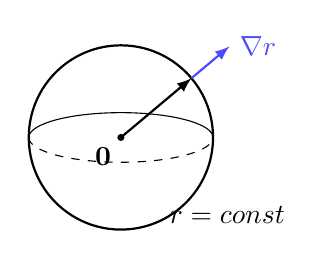
\begin{tikzpicture}[scale=0.9, >=latex]
			\draw[thick] (0,0) circle (1.3);
			\draw[dashed] (-1.3,0) arc[start angle=180, end angle=360, x radius=1.3, y radius=0.35];
			\draw (-1.3,0) arc[start angle=180, end angle=0, x radius=1.3, y radius=0.35];
			\fill (0,0) circle (0.05);
			\draw[->, thick] (0,0) -- ({1.3*cos(40)},{1.3*sin(40)});
			\draw[->, thick, blue!70] ({1.3*cos(40)},{1.3*sin(40)}) -- ++({0.7*cos(40)},{0.7*sin(40)})
			node[right]{$\nabla r$};
			\node[below left] at (0,0) {$\mathbf{0}$};
			\node at (1.5,-1.1) {$r = \text{const}$};
		\end{tikzpicture}
  \end{center}

  Either way,
  \[
    -\nabla V = -\frac{GMm}{r^2}\,\hat{\mathbf{x}} = \mathbf{F}
  \]
\end{example}

\subsection{Line Integrals}

\begin{example}

  A line integral is used to define quantities like the work done by a force field along a curve.

  \begin{center}
    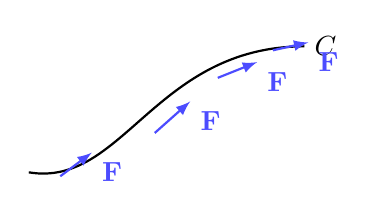
\begin{tikzpicture}[scale=1, >=latex]
			\draw[thick] (-2,-0.6) .. controls (-0.8,-0.8) and (-0.4,1) .. (1.5,1)
			node[right]{$C$};
			\foreach \x/\y/\dx/\dy in {
					-1.6/-0.65/0.4/0.3,
					-0.4/-0.1/0.45/0.4,
					0.4/0.6/0.5/0.2,
					1.1/0.95/0.45/0.1
				} {
					\draw[->, thick, blue!70] (\x,\y) -- ++(\dx,\dy) node[below right]{$\mathbf{F}$};
				}
		\end{tikzpicture}
  \end{center}
\end{example}

\subsubsection{Line Integral of a Scalar Function}

\begin{definition}{Line Integral of a Scalar Function}{line-integral-scalar}
  Let $C$ be a smooth curve parametrized by $x(t),\,y(t)$ for $t\in[a,b]$,
  and let $f(x,y)$ be a scalar function. The \emph{line integral of $f$ along $C$} is
  \[
    \int_C f(x,y)\dd{s}
    = \int_a^b f(x(t),\,y(t))\,
    \underbrace{\sqrt{\left(\frac{\dd{x}}{\dd{t}}\right)^2 + \left(\frac{\dd{y}}{\dd{t}}\right)^2}\dd{t}}_{\dd{s}}
  \]
\end{definition}

\textbf{Interpretation of $\dd{s}$.} Along a small piece of the curve from $\mathbf{r}(t)$
to $\mathbf{r}(t+\dd{t})$, the displacement has horizontal component $\dd{x}$ and vertical
component $\dd{y}$, so the arclength element satisfies
\[
  \dd{s} = \sqrt{(\dd{x})^2 + (\dd{y})^2}
  = \sqrt{\left(\frac{\dd{x}}{\dd{t}}\right)^2 + \left(\frac{\dd{y}}{\dd{t}}\right)^2}\dd{t}
  = \lVert\mathbf{r}'(t)\rVert\dd{t}
\]
where $\mathbf{r}(t) = \ve{x(t),\,y(t)}$ is parametrized curve and $\mathbf{r}'(t) = \ve{\dfrac{\dd{x}}{\dd{t}},\,\dfrac{\dd{y}}{\dd{t}}}$
is the velocity vector.

\begin{center}
  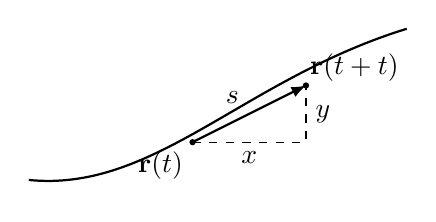
\begin{tikzpicture}[scale=1.6, >=latex]
		\draw[thick] (-1.5,-0.3) .. controls (-0.5,-0.4) and (0.2,0.5) .. (1.5,0.9);
		\fill (-0.2,0) circle (0.025) node[below left]{$\mathbf{r}(t)$};
		\fill (0.7,0.45) circle (0.025) node[above right=-2pt]{$\mathbf{r}(t+\dd{t})$};
		\draw[dashed] (-0.2,0) -- (0.7,0) -- (0.7,0.45);
		\node[below] at (0.25,0) {$\dd{x}$};
		\node[right] at (0.7,0.22) {$\dd{y}$};
		\draw[->, thick] (-0.2,0) -- (0.7,0.45) node[midway, above left]{$\dd{s}$};
	\end{tikzpicture}
\end{center}

\begin{note}
  $\dd{s} = \lVert\mathbf{r}'\rVert\dd{t}$, $\lVert\mathbf{r}'\rVert$ is the Jacobian.
\end{note}

\textbf{Geometric meaning.} For $f\geq 0$, the integral $\int_C f(x,y)\dd{s}$ is the
area of the ``curtain'' standing above the curve $C$ in the $xy$-plane, with height
$z = f(x,y)$.

\begin{center}
  \tdplotsetmaincoords{70}{120}
  \begin{tikzpicture}[tdplot_main_coords, scale=1.2, >=latex]
		\draw[->] (0,0,0) -- (2.4,0,0) node[below]{$x$};
		\draw[->] (0,0,0) -- (0,2.4,0) node[right]{$y$};
		\draw[->] (0,0,0) -- (0,0,2) node[above]{$z$};

		\draw[thick, domain=0:3.14159, smooth, samples=40, variable=\t]
		plot ({1.6*cos(\t r)}, {1.6*sin(\t r)}, 0);

		\draw[thick, blue!70, domain=0:3.14159, smooth, samples=40, variable=\t]
		plot ({1.6*cos(\t r)}, {1.6*sin(\t r)}, {0.6+0.4*sin(\t r)});

		\foreach \t in {0.3, 0.7, 1.1, 1.5708, 2.0, 2.4, 2.8} {
				\draw[gray!60]
				({1.6*cos(\t r)}, {1.6*sin(\t r)}, 0)
				-- ({1.6*cos(\t r)}, {1.6*sin(\t r)}, {0.6+0.4*sin(\t r)});
			}
		\node at (1.9,1.3,1.2) {$z = f(x,y)$};
		\node[below] at (-1.6,0.1,0) {$C$};
	\end{tikzpicture}
\end{center}

\begin{example}
  Evaluate $\displaystyle\int_C (2 + x^2 y)\dd{s}$ where $C$ is the upper half of
  the unit circle $x^2 + y^2 = 1$.

  Parametrize: $\mathbf{r}(t) = \ve{\cos t,\,\sin t}$, $t\in[0,\pi]$.

  Velocity: $\mathbf{r}'(t) = \ve{-\sin t,\,\cos t}$, so $\lVert\mathbf{r}'(t)\rVert = 1$.

  \begin{align*}
    \int_C (2 + x^2 y)\dd{s}
     & = \int_0^{\pi} (2 + \cos^2 t \sin t)\cdot 1\dd{t} \\
     & = 2\pi + \int_0^{\pi} \cos^2 t \sin t\dd{t}       \\
     & = 2\pi + \frac{2}{3}
  \end{align*}
\end{example}

\subsubsection{Line Integrals with Respect to $x$ and $y$}

Instead of the arclength element $\dd{s}$, integrate against the projections of $\mathbf{r}$
onto the $x$- or $y$-axis:
\[
  \int_C f\dd{x} = \int_a^b f(x(t),\,y(t))\,x'(t)\dd{t},
  \qquad
  \int_C f\dd{y} = \int_a^b f(x(t),\,y(t))\,y'(t)\dd{t}
\]

These are usually combined. Writing $\mathbf{F} = \ve{P,\,Q}$ and $\dd{\mathbf{r}} = \ve{\dd{x},\,\dd{y}}$,
\[
  \int_C P\dd{x} + \int_C Q\dd{y}
  = \int_C P\dd{x} + Q\dd{y}
  = \int_C \ve{P,\,Q}\cdot\ve{\dd{x},\,\dd{y}}
\]

\subsubsection{Line Integral of a Vector Field}

\begin{definition}{Line Integral of a Vector Field}{line-integral-vector}
  Let $\mathbf{F}$ be a continuous vector field defined on a smooth curve $C$
  parametrized by $\mathbf{r}(t)$, $t\in[a,b]$. The \emph{line integral of $\mathbf{F}$
    along $C$} is
  \[
    \int_C \mathbf{F}\cdot \dd{\mathbf{r}}
    = \int_a^b \mathbf{F}(\mathbf{r}(t))\cdot\mathbf{r}'(t)\dd{t}
  \]
\end{definition}

\textbf{Geometric interpretation.} Let $\mathbf{T}(t) = \mathbf{r}'(t)/\lVert\mathbf{r}'(t)\rVert$
be the unit tangent. Since $\mathbf{r}'(t)\dd{t} = \mathbf{T}(t)\dd{s}$,
\[
  \int_C \mathbf{F}\cdot \dd{\mathbf{r}}
  = \int_C \mathbf{F}\cdot\mathbf{T}\dd{s}
\]
i.e.\ integrate the tangential component of $\mathbf{F}$ along $C$.

\begin{example}[Work in physics]
  If $\mathbf{F}$ is a force field and $C$ is the path of a particle, then
  $\int_C \mathbf{F}\cdot \dd{\mathbf{r}}$ is the work done by $\mathbf{F}$ on the particle.
\end{example}

\textbf{Orientation.} For a vector line integral, reversing the direction of $C$
flips the sign:
\[
  \int_{-C} \mathbf{F}\cdot \dd{\mathbf{r}} = -\int_C \mathbf{F}\cdot \dd{\mathbf{r}}
\]

\begin{remark}
  A scalar line integral $\int_C f\dd{s}$ depends only on the \emph{shape} of $C$;
  a vector line integral $\int_C \mathbf{F}\cdot \dd{\mathbf{r}}$ depends on the shape
  \emph{and} the direction of traversal.
\end{remark}

\textbf{Additivity.} Analogous to $\int_a^b f\dd{x} = \int_a^c f\dd{x} + \int_c^b f\dd{x}$:
if $C = C_1 + C_2$ is a union of curves traversed in sequence,
\[
  \int_{C_1} \mathbf{F}\cdot \dd{\mathbf{r}} + \int_{C_2} \mathbf{F}\cdot \dd{\mathbf{r}}
  = \int_{C_1 + C_2} \mathbf{F}\cdot \dd{\mathbf{r}}
\]

\begin{center}
  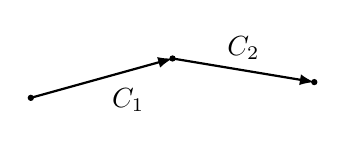
\begin{tikzpicture}[scale=1, >=latex]
		\draw[->, thick] (-2,0) -- (-0.2,0.5) node[midway, below right]{$C_1$};
		\draw[->, thick] (-0.2,0.5) -- (1.6,0.2) node[midway, above]{$C_2$};
		\fill (-2,0) circle (0.04);
		\fill (-0.2,0.5) circle (0.04);
		\fill (1.6,0.2) circle (0.04);
	\end{tikzpicture}
\end{center}

\begin{example}
  Evaluate $\displaystyle\int_C \mathbf{F}\cdot \dd{\mathbf{r}}$ where
  $\mathbf{F}(x,y,z) =
    \begin{bmatrix}
      y+z \\ x+z \\ x+y
    \end{bmatrix}
  $ and $C$
  is the broken path $(0,0,0)\to(1,0,1)\to(0,1,2)$.

  \textbf{Step 1 — Parametrize $C$.}

  \emph{Trick:} interpolate linearly from the start
  point (at $t=0$) to the end point (at $t=1$):
  \[
    \mathbf{r}(t) = (1-t)\,\mathbf{p}_{\text{start}} + t\,\mathbf{p}_{\text{end}},
    \qquad t\in[0,1]
  \]

  \[
    C_1\colon\quad
    \mathbf{r}_1(t) = (1-t)
    \begin{bmatrix}
      0 \\0\\0
    \end{bmatrix}
    + t
    \begin{bmatrix}
      1 \\0\\1
    \end{bmatrix}
    =
    \begin{bmatrix}
      t \\0\\t
    \end{bmatrix}
    ,
    \qquad
    \mathbf{r}_1'(t) =
    \begin{bmatrix}
      1 \\0\\1
    \end{bmatrix}
  \]
  \[
    C_2\colon\quad
    \mathbf{r}_2(t) = (1-t)
    \begin{bmatrix}
      1 \\0\\1
    \end{bmatrix}
    + t
    \begin{bmatrix}
      0 \\1\\2
    \end{bmatrix}
    =
    \begin{bmatrix}
      1-t \\t\\1+t
    \end{bmatrix}
    ,
    \qquad
    \mathbf{r}_2'(t) =
    \begin{bmatrix}
      -1 \\1\\1
    \end{bmatrix}
  \]

  \textbf{Step 2 — Evaluate piecewise.}

  On $C_1$, with $x=t,\,y=0,\,z=t$:
  \[
    \mathbf{F}(\mathbf{r}_1(t))
    =
    \begin{bmatrix}
      0+t \\t+t\\t+0
    \end{bmatrix}
    =
    \begin{bmatrix}
      t \\2t\\t
    \end{bmatrix}
  \]
  \[
    \int_{C_1}\mathbf{F}\cdot \dd{\mathbf{r}}
    = \int_0^1
    \begin{bmatrix}
      t \\2t\\t
    \end{bmatrix}
    \cdot
    \begin{bmatrix}
      1 \\0\\1
    \end{bmatrix}
    \dd{t}
    = \int_0^1 2t\dd{t} = 1
  \]

  On $C_2$, with $x=1-t,\,y=t,\,z=1+t$:
  \[
    \mathbf{F}(\mathbf{r}_2(t))
    =
    \begin{bmatrix}
      t+(1+t) \\(1-t)+(1+t)\\(1-t)+t
    \end{bmatrix}
    =
    \begin{bmatrix}
      1+2t \\2\\1
    \end{bmatrix}
  \]
  \[
    \int_{C_2}\mathbf{F}\cdot \dd{\mathbf{r}}
    = \int_0^1
    \begin{bmatrix}
      1+2t \\2\\1
    \end{bmatrix}
    \cdot
    \begin{bmatrix}
      -1 \\1\\1
    \end{bmatrix}
    \dd{t}
    = \int_0^1 (-(1+2t)+2+1)\dd{t}
    = \int_0^1 (2-2t)\dd{t} = 1
  \]

  Total:
  \[
    \int_C \mathbf{F}\cdot \dd{\mathbf{r}}
    = \int_{C_1}\mathbf{F}\cdot \dd{\mathbf{r}} + \int_{C_2}\mathbf{F}\cdot \dd{\mathbf{r}}
    = 1 + 1 = 2
  \]
\end{example}

\subsection{Fundamental Theorem for Line Integrals}

Analogue to the single-variable FTC: think of $\nabla f$ as the ``derivative'' of $f$.

\begin{remark}
  For $f\colon\R^n\to\R$,
  \[
    \nabla f = \ve{\pd{f}{x},\,\pd{f}{y},\,\ldots}\colon \R^n\to\R^n
  \]
  is itself a vector field.
\end{remark}

\begin{remark}
  For $\mathbf{F}\colon\R^n\to\R^n$ a vector field, we say $\mathbf{F}$ is conservative if
  $\mathbf{F} = \nabla f$ for some scalar function $f\colon\R^n\to\R$.
\end{remark}

\begin{theorem}{Fundamental Theorem for Line Integrals}{ftli}
  Let $C$ be a smooth curve given by $\mathbf{r}(t)$, $t\in[a,b]$, and let $f$ be a
  differentiable scalar function whose gradient $\nabla f$ is continuous on $C$. Then
  \[
    \int_C \nabla f\cdot \dd{\mathbf{r}} = f(\mathbf{r}(b)) - f(\mathbf{r}(a))
  \]
\end{theorem}

\begin{proof}

  \begin{remark}
    Note that $\mathbf{r}(t) =
      \begin{bmatrix}
        x(t) \\y(t)\\z(t)
      \end{bmatrix}
    $.
  \end{remark}

  By the multivariable chain rule,
  \[
    \frac{\dd{}}{\dd{t}}f(\mathbf{r}(t))
    = \pd{f}{x}\frac{\dd{x}}{\dd{t}} + \pd{f}{y}\frac{\dd{y}}{\dd{t}} + \cdots
    =
    \begin{bmatrix}
      \dfrac{\partial f}{\partial x} \\[8pt] \dfrac{\partial f}{\partial y} \\[8pt] \vdots
    \end{bmatrix}
    \cdot
    \begin{bmatrix}
      \dfrac{\dd{x}}{\dd{t}} \\[8pt] \dfrac{\dd{y}}{\dd{t}} \\[8pt] \vdots
    \end{bmatrix}
    = \nabla f(\mathbf{r}(t))\cdot\mathbf{r}'(t)
  \]
  Therefore
  \[
    \int_C \nabla f\cdot \dd{\mathbf{r}}
    = \int_a^b \nabla f(\mathbf{r}(t))\cdot\mathbf{r}'(t)\dd{t}
    = \int_a^b \frac{\dd{}}{\dd{t}}f(\mathbf{r}(t))\dd{t}
    = f(\mathbf{r}(b)) - f(\mathbf{r}(a))
  \]
\end{proof}

As a result, on a conservative vector field $\mathbf{F} = \nabla f$, the line integral $\int_C \mathbf{F}\cdot \dd{\mathbf{r}}$ is
independent of the path $C$ and depends only on the endpoints $\mathbf{r}(a)$ and $\mathbf{r}(b)$.

\begin{example}[Work done by gravity]
  Find the work done by the gravitational field
  \[
    \mathbf{F}(\mathbf{x}) = -\frac{GMm}{\lVert\mathbf{x}\rVert^3}\mathbf{x}
  \]
  on a particle moving from $\mathbf{x}_0 = (3,4,12)$ to $\mathbf{x}_1 = (2,2,1)$.

  Recall the potential $V(\mathbf{x}) = -\dfrac{GMm}{\lVert\mathbf{x}\rVert}$ satisfies $\mathbf{F} = -\nabla V$, so by FTLI,
  \[
    \int_C \mathbf{F}\cdot \dd{\mathbf{r}}
    = -\int_C \nabla V\cdot \dd{\mathbf{r}}
    = -\bigl(V(\mathbf{x}_1) - V(\mathbf{x}_0)\bigr)
    = \frac{GMm}{\lVert\mathbf{x}_1\rVert} - \frac{GMm}{\lVert\mathbf{x}_0\rVert}
  \]
  Compute norms:
  \[
    \lVert\mathbf{x}_0\rVert = \sqrt{9+16+144} = 13,\qquad
    \lVert\mathbf{x}_1\rVert = \sqrt{4+4+1} = 3
  \]
  Therefore
  \[
    \int_C \mathbf{F}\cdot \dd{\mathbf{r}}
    = GMm\left(\frac{1}{3} - \frac{1}{13}\right)
    = \frac{10\,GMm}{39}
  \]
\end{example}

\subsection{Independence of Path}

\begin{theorem}{Independence of Path for Conservative Fields}{path-independent-conservative}
  If $\mathbf{F} = \nabla f$ is conservative on a domain $D$, then
  \[
    \int_{C_1}\mathbf{F}\cdot \dd{\mathbf{r}}
    =
    \int_{C_2}\mathbf{F}\cdot \dd{\mathbf{r}}
  \]
  whenever $C_1$ and $C_2$ are curves in $D$ with the same initial and terminal points.
\end{theorem}

\begin{proof}
  By the Fundamental Theorem for Line Integrals,
  \[
    \int_{C_i}\mathbf{F}\cdot \dd{\mathbf{r}}
    =
    \int_{C_i}\nabla f\cdot \dd{\mathbf{r}}
    =
    f(\text{terminal point}) - f(\text{initial point})
  \]
  for $i=1,2$. The endpoints are the same, so the integrals are equal.
\end{proof}

\begin{theorem}{Zero Circulation and Path Independence}{zero-circulation-path-independent}
  Let $\mathbf{F}$ be continuous on an open connected region $D$. Then
  \[
    \int_C \mathbf{F}\cdot \dd{\mathbf{r}}
    \text{ is independent of path in }D
    \quad\Longleftrightarrow\quad
    \oint_C \mathbf{F}\cdot \dd{\mathbf{r}} = 0
    \text{ for every closed loop }C\subset D.
  \]
\end{theorem}

\begin{proof}
  Suppose the line integral is independent of path. If $C$ is a closed loop, then
  its initial and terminal points are the same, so
  \[
    \oint_C \mathbf{F}\cdot \dd{\mathbf{r}}=0.
  \]

  Conversely, suppose every closed loop has zero circulation. If $C_1$ and $C_2$
  have the same initial and terminal points, then $C=C_1+(-C_2)$ is a closed loop.
  Thus
  \[
    0
    =
    \oint_C \mathbf{F}\cdot \dd{\mathbf{r}}
    =
    \int_{C_1}\mathbf{F}\cdot \dd{\mathbf{r}}
    +
    \int_{-C_2}\mathbf{F}\cdot \dd{\mathbf{r}}
    =
    \int_{C_1}\mathbf{F}\cdot \dd{\mathbf{r}}
    -
    \int_{C_2}\mathbf{F}\cdot \dd{\mathbf{r}}.
  \]
  Hence the two path integrals are equal.
\end{proof}

\begin{center}
  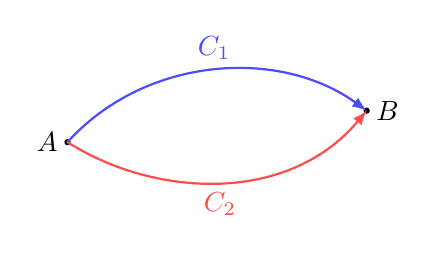
\begin{tikzpicture}[scale=1, >=latex]
		\fill (-2,0) circle (0.04) node[left]{$A$};
		\fill (1.8,0.4) circle (0.04) node[right]{$B$};
		\draw[->, thick, blue!70]
		(-2,0) .. controls (-1,1.1) and (0.7,1.2) .. (1.8,0.4)
		node[midway, above]{$C_1$};
		\draw[->, thick, red!70]
		(-2,0) .. controls (-0.9,-0.7) and (0.8,-0.8) .. (1.8,0.4)
		node[midway, below]{$C_2$};
	\end{tikzpicture}
\end{center}

\begin{theorem}{Path Independence and Conservative Fields}{path-independent-conservative-iff}
  Let $\mathbf{F}$ be continuous on an open connected region $D$. Then
  \[
    \int_C \mathbf{F}\cdot \dd{\mathbf{r}}
    \text{ is independent of path in }D
    \quad\Longleftrightarrow\quad
    \mathbf{F}\text{ is conservative on }D.
  \]
\end{theorem}

\begin{remark}
  On an open connected domain $D$,
  \[
    \mathbf{F} \text{ is conservative} \iff \int_C \mathbf{F} \cdot \dd{\mathbf{r}} \text{ is independent of path} \,, \forall \text{ path } C \iff \oint_C \mathbf{F} \cdot \dd{\mathbf{r}} = 0 \,, \forall \text{ loop } C
  \]
  and each of these implies $P_y = Q_x$ (with continuous first partials). The converse $P_y = Q_x \implies \mathbf{F}$ conservative holds when $D$ is simply connected.
\end{remark}

\begin{definition}{Simply Connected Region}{simply-connected}
  A region $D$ is \emph{simply connected} if every closed loop in $D$ can be
  continuously shrunk to a point while staying inside $D$.
\end{definition}

\begin{center}
  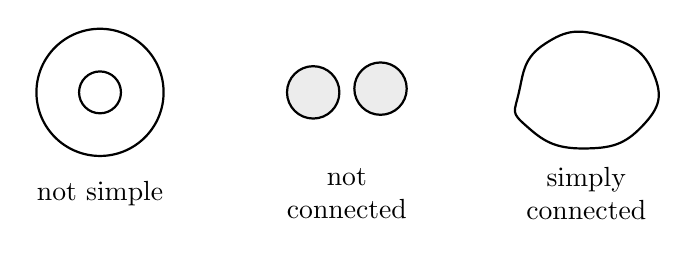
\begin{tikzpicture}[scale=0.95, >=latex]
		\begin{scope}
			\draw[thick] (0,0) circle (0.85);
			\fill[white] (0,0) circle (0.28);
			\draw[thick] (0,0) circle (0.28);
			\node[align=center] at (0,-1.35) {not simple};
		\end{scope}

		\begin{scope}[xshift=3.2cm]
			\filldraw[fill=gray!15, draw=black, thick] (-0.35,0) circle (0.35);
			\filldraw[fill=gray!15, draw=black, thick] (0.55,0.05) circle (0.35);
			\node[align=center] at (0.1,-1.35) {not\\connected};
		\end{scope}

		\begin{scope}[xshift=6.5cm]
			\draw[thick] plot[smooth cycle, tension=0.9]
			coordinates {(-0.9,0) (-0.55,0.65) (0.25,0.75) (0.9,0.25)
					(0.75,-0.45) (-0.05,-0.75) (-0.8,-0.45)};
			\node[align=center] at (0,-1.35) {simply\\connected};
		\end{scope}
	\end{tikzpicture}
\end{center}

\begin{theorem}{Component Test for Conservative Vector Fields}{component-test-conservative}

  For vector field $\mathbf{F}(x, y)=
    \begin{bmatrix}
      P(x, y) \\Q(x, y)
    \end{bmatrix}
  $ with continuous first-order partials,

  \[
    \mathbf{F} \text{ is conservative} \implies \pd{P}{y} = \pd{Q}{x}.
  \]

  If $D$ is simply connected, the converse also holds:
  \[
    \pd{P}{y} = \pd{Q}{x}
    \implies
    \mathbf{F}\text{ is conservative on }D.
  \]

\end{theorem}

\begin{proof}
  Suppose $\mathbf{F} = \nabla f$ for some scalar function $f$. Then
  \[
    \mathbf{F} =
    \begin{bmatrix}
      P \\ Q
    \end{bmatrix}
    =
    \begin{bmatrix}
      f_x \\ f_y
    \end{bmatrix}
  \]
  By Clairaut's theorem on equality of mixed partials, $f_{xy} = f_{yx}$,
  \[
    \pd{P}{y} = f_{xy} = f_{yx} = \pd{Q}{x}
  \]

  For the converse, assume $D$ is simply connected and $\pd{P}{y}=\pd{Q}{x}$.
  For any closed loop $C$ in $D$, let $R$ be the region inside $C$. Since $D$ has
  no holes, $R\subset D$. By Green's theorem,
  \[
    \oint_C \mathbf{F}\cdot \dd{\mathbf{r}}
    =
    \oint_C P\dd{x}+Q\dd{y}
    =
    \iint_R \left(\pd{Q}{x}-\pd{P}{y}\right)\dd{A}
    =
    0.
  \]
  Thus every closed loop has zero circulation, so the line integral is independent
  of path by Theorem~\ref{thm:zero-circulation-path-independent}. Hence
  $\mathbf{F}$ is conservative by Theorem~\ref{thm:path-independent-conservative-iff}.
\end{proof}

\begin{center}
  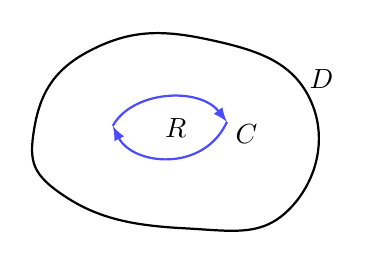
\begin{tikzpicture}[scale=1, >=latex]
		\draw[thick] plot[smooth cycle, tension=0.8]
		coordinates {(-1.8,0.1) (-1.1,1.1) (0.4,1.25) (1.7,0.5)
				(1.45,-0.9) (0.1,-1.15) (-1.4,-0.75)};
		\draw[->, thick, blue!70] (-0.8,0.15)
		.. controls (-0.55,0.6) and (0.3,0.65) .. (0.65,0.2);
		\draw[->, thick, blue!70] (0.65,0.2)
		.. controls (0.35,-0.45) and (-0.55,-0.35) .. (-0.8,0.15);
		\node at (0,0.12) {$R$};
		\node at (1.85,0.75) {$D$};
		\node at (0.9,0.05) {$C$};
	\end{tikzpicture}
\end{center}

\subsection{Green's Theorem}

\textbf{Orientation of a simple closed curve.} Let $C$ be a simple closed curve
with unit tangent $\mathbf{T}$ and inward unit normal $\mathbf{N}$.
\begin{itemize}
  \item If $\mathbf{N}$ is $90^\circ$ counterclockwise from $\mathbf{T}$
        (equivalently, $C$ is traversed counterclockwise), $C$ is
        \emph{positively oriented}.
  \item If $\mathbf{N}$ is $90^\circ$ clockwise from $\mathbf{T}$
        (equivalently, $C$ is traversed clockwise), $C$ is
        \emph{negatively oriented}.
\end{itemize}

\begin{center}
  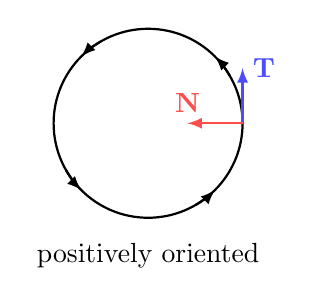
\begin{tikzpicture}[scale=1, >=latex]
		\draw[thick] (0,0) circle (1.2);
		\foreach \a in {30, 120, 210, 300} {
				\draw[->, thick] ({1.2*cos(\a)},{1.2*sin(\a)})
				arc[start angle=\a, end angle=\a+15, radius=1.2];
			}
		\draw[->, thick, blue!70] (1.2,0) -- (1.2,0.7) node[right]{$\mathbf{T}$};
		\draw[->, thick, red!70] (1.2,0) -- (0.5,0) node[above]{$\mathbf{N}$};
		\node[below] at (0,-1.4) {positively oriented};
	\end{tikzpicture}
  \qquad\qquad
  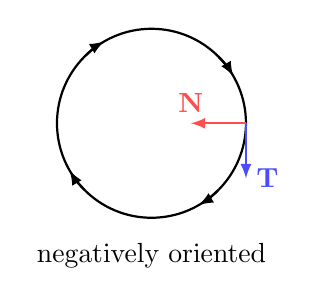
\begin{tikzpicture}[scale=1, >=latex]
		\draw[thick] (0,0) circle (1.2);
		\foreach \a in {30, 120, 210, 300} {
				\draw[<-, thick] ({1.2*cos(\a)},{1.2*sin(\a)})
				arc[start angle=\a, end angle=\a+15, radius=1.2];
			}
		\draw[->, thick, blue!70] (1.2,0) -- (1.2,-0.7) node[right]{$\mathbf{T}$};
		\draw[->, thick, red!70] (1.2,0) -- (0.5,0) node[above]{$\mathbf{N}$};
		\node[below] at (0,-1.4) {negatively oriented};
	\end{tikzpicture}
\end{center}

\begin{theorem}{Green's Theorem}{green}
  Let $C$ be a positively oriented, piecewise-smooth simple closed curve in
  $\R^2$, and let $D$ be the region bounded by $C$. If
  $\mathbf{F} =
    \begin{bmatrix}
      P \\ Q
    \end{bmatrix}
  $ has continuous partial
  derivatives on an open region containing $D$, then
  \[
    \oint_C \mathbf{F}\cdot \dd{\mathbf{r}}
    = \int_C P\dd{x} + Q\dd{y}
    = \iint_D \left(\pd{Q}{x} - \pd{P}{y}\right)\dd{A}
  \]
\end{theorem}

\begin{center}
  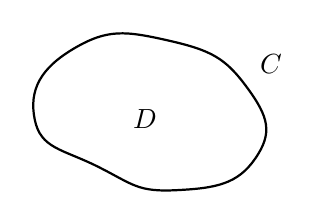
\begin{tikzpicture}[scale=1, >=latex]
		\draw[thick] plot[smooth cycle, tension=0.9]
		coordinates {(-1.4,0) (-0.9,0.9) (0.3,1) (1.3,0.4) (1.4,-0.5) (0.4,-0.9) (-0.6,-0.6)};
		\node at (0,0) {$D$};
		\node at (1.6,0.7) {$C$};
	\end{tikzpicture}
\end{center}

Green's theorem can turn a potentially difficult to calculate line integral into a double integral.

\begin{remark}
  Mnemonic:
  \[
    \pd{Q}{x} - \pd{P}{y}
    = \det
    \begin{bmatrix}
      \partial/\partial x & \partial/\partial y \\
      P                   & Q
    \end{bmatrix}
  \]
\end{remark}

\begin{example}
  Evaluate $\displaystyle\int_C x^4\dd{x} + xy\dd{y}$ where $C$ is the triangle
  with vertices $(0,0)\to(1,0)\to(0,1)\to(0,0)$.

  \begin{center}
    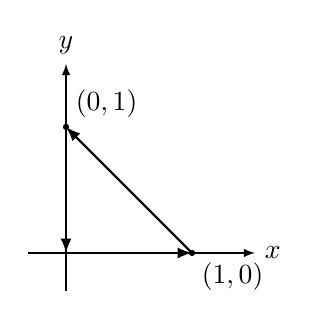
\begin{tikzpicture}[scale=1.6, >=latex]
			\draw[->] (-0.3,0) -- (1.5,0) node[right]{$x$};
			\draw[->] (0,-0.3) -- (0,1.5) node[above]{$y$};
			\draw[->, thick] (0,0) -- (1,0);
			\draw[->, thick] (1,0) -- (0,1);
			\draw[->, thick] (0,1) -- (0,0);
			\fill (1,0) circle (0.025) node[below right]{$(1,0)$};
			\fill (0,1) circle (0.025) node[above right]{$(0,1)$};
		\end{tikzpicture}
  \end{center}

  The triangle is traversed counterclockwise, so Green's theorem applies. With
  $P = x^4$ and $Q = xy$,
  \[
    \pd{Q}{x} - \pd{P}{y} = y - 0 = y
  \]
  \begin{align*}
    \int_C x^4\dd{x} + xy\dd{y}
     & = \iint_D y\dd{A}
    = \int_0^1\!\int_0^{1-x} y\dd{y}\dd{x} \\
     & = \int_0^1 \frac{(1-x)^2}{2}\dd{x}
    = \frac{1}{6}
  \end{align*}
\end{example}

\begin{example}
  Let
  \[
    \mathbf{F}(x,y)
    =
    \frac{1}{x^2+y^2}
    \begin{bmatrix}
      -y \\
      x
    \end{bmatrix}
    =
    \begin{bmatrix}
      P \\
      Q
    \end{bmatrix}
    .
  \]
  Show that a positively oriented circle around the origin satisfies
  \[
    \oint_C \mathbf{F}\cdot\dd{\mathbf{r}} = 2\pi.
  \]

  First check the component test:
  \[
    \pd{Q}{x}
    =
    \pd{}{x}\left(\frac{x}{x^2+y^2}\right)
    =
    \frac{y^2-x^2}{(x^2+y^2)^2},
  \]
  \[
    \pd{P}{y}
    =
    \pd{}{y}\left(\frac{-y}{x^2+y^2}\right)
    =
    \frac{y^2-x^2}{(x^2+y^2)^2}.
  \]
  Thus $\pd{Q}{x}=\pd{P}{y}$, but this does not imply $\mathbf{F}$ is conservative
  on $\R^2\setminus\{(0,0)\}$ because the domain has a hole and is not simply
  connected.

  Consider the circle $C$ with radius $r>0$:
  \[
    \mathbf{r}(t)=\ve{r\cos t,\, r\sin t},
    \qquad 0\leq t\leq 2\pi.
  \]
  Then
  \[
    \mathbf{r}'(t)=\ve{-r\sin t,\, r\cos t},
    \qquad
    \mathbf{F}(\mathbf{r}(t))
    =
    \begin{bmatrix}
      -\dfrac{\sin t}{r} \\[6pt]
      \dfrac{\cos t}{r}
    \end{bmatrix}
    .
  \]
  Therefore
  \[
    \oint_C \mathbf{F}\cdot\dd{\mathbf{r}}
    =
    \int_0^{2\pi}
    \begin{bmatrix}
      -\dfrac{\sin t}{r} \\[6pt]
      \dfrac{\cos t}{r}
    \end{bmatrix}
    \cdot
    \begin{bmatrix}
      -r\sin t \\
      r\cos t
    \end{bmatrix}
    \dd{t}
    =
    \int_0^{2\pi} 1\dd{t}
    =
    2\pi.
  \]

  \begin{center}
    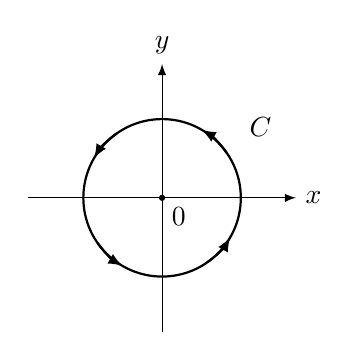
\begin{tikzpicture}[scale=1, >=latex]
			\draw[->] (-1.7,0) -- (1.7,0) node[right]{$x$};
			\draw[->] (0,-1.7) -- (0,1.7) node[above]{$y$};
			\draw[thick] (0,0) circle (1);
			\foreach \a in {35, 125, 215, 305} {
					\draw[->, thick] ({cos(\a)},{sin(\a)})
					arc[start angle=\a, end angle=\a+25, radius=1];
				}
			\fill (0,0) circle (0.04) node[below right]{$0$};
			\node at (1.25,0.9) {$C$};
		\end{tikzpicture}
  \end{center}
\end{example}

\begin{theorem}{Extended Green's Theorem}{extended-green}
  Let $D$ be a region whose positively oriented boundary consists of an outer
  curve $C_{\text{out}}$ and an inner curve $C_{\text{in}}$ around a hole. If
  $\mathbf{F}=
    \begin{bmatrix}
      P \\Q
    \end{bmatrix}
  $ has continuous partial derivatives
  on an open region containing $D$, then
  \[
    \iint_D \left(\pd{Q}{x}-\pd{P}{y}\right)\dd{A}
    =
    \oint_{C_{\text{out}}}\mathbf{F}\cdot\dd{\mathbf{r}}
    -
    \oint_{C_{\text{in}}}\mathbf{F}\cdot\dd{\mathbf{r}},
  \]
  where both $C_{\text{out}}$ and $C_{\text{in}}$ are written with
  counterclockwise orientation.
\end{theorem}

\begin{center}
  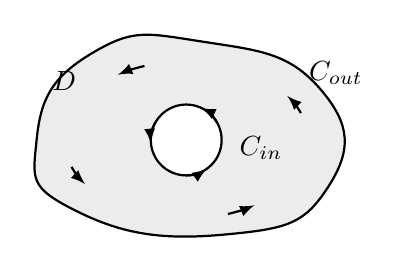
\begin{tikzpicture}[scale=1, >=latex]
		\fill[gray!15, even odd rule] plot[smooth cycle, tension=0.9]
		coordinates {(-1.9,0) (-1.2,1.1) (0.2,1.25) (1.7,0.65)
				(1.8,-0.6) (0.5,-1.2) (-1.4,-0.9)}
		(0,0) circle (0.45);
		\draw[thick] plot[smooth cycle, tension=0.9]
		coordinates {(-1.9,0) (-1.2,1.1) (0.2,1.25) (1.7,0.65)
				(1.8,-0.6) (0.5,-1.2) (-1.4,-0.9)};
		\draw[thick] (0,0) circle (0.45);
		\foreach \a in {20, 110, 200, 290} {
				\draw[->, thick] ({1.55*cos(\a)},{1.0*sin(\a)})
				arc[start angle=\a, end angle=\a+14, x radius=1.55, y radius=1.0];
			}
		\foreach \a in {30, 150, 270} {
				\draw[->, thick] ({0.45*cos(\a)},{0.45*sin(\a)})
				arc[start angle=\a, end angle=\a+35, radius=0.45];
			}
		\node at (-1.55,0.75) {$D$};
		\node at (1.9,0.85) {$C_{\text{out}}$};
		\node at (0.95,-0.1) {$C_{\text{in}}$};
	\end{tikzpicture}
\end{center}

\begin{example}

  For the vector field above, if $C$ is any positively oriented simple closed curve
  containing the origin, choose a small circle $C_{\text{in}}$ around the origin
  inside $C$. On the annular region between the curves,
  \[
    \pd{Q}{x}-\pd{P}{y}=0.
  \]
  By Theorem~\ref{thm:extended-green},
  \[
    0
    =
    \oint_C \mathbf{F}\cdot\dd{\mathbf{r}}
    -
    \oint_{C_{\text{in}}}\mathbf{F}\cdot\dd{\mathbf{r}},
  \]
  so
  \[
    \oint_C \mathbf{F}\cdot\dd{\mathbf{r}}
    =
    \oint_{C_{\text{in}}}\mathbf{F}\cdot\dd{\mathbf{r}}
    =
    2\pi.
  \]

\end{example}

\begin{example}[Area of an ellipse]
  Find the area enclosed by $\dfrac{x^2}{a^2}+\dfrac{y^2}{b^2}=1$.

  Let $D$ be the region enclosed. Then
  \[
    \operatorname{Area}(D) = \iint_D 1\dd{A}.
  \]
  Pick $\mathbf{F}=
    \begin{bmatrix}
      P \\Q
    \end{bmatrix}
  $ with $\pd{Q}{x}-\pd{P}{y}=1$. By Green's theorem,
  \[
    \operatorname{Area}(D)
    = \iint_D \left(\pd{Q}{x}-\pd{P}{y}\right)\dd{A}
    = \oint_C \mathbf{F}\cdot\dd{\mathbf{r}}.
  \]
  One choice is $\mathbf{F}=
    \begin{bmatrix}
      0 \\x
    \end{bmatrix}
  $, which gives $\pd{Q}{x}-\pd{P}{y}=1$.

  Parametrize the boundary:
  \[
    C\colon\quad \mathbf{r}(t)=\ve{a\cos t,\,b\sin t},\qquad t\in[0,2\pi],
  \]
  so $\mathbf{r}'(t)=\ve{-a\sin t,\,b\cos t}$ and $\mathbf{F}(\mathbf{r}(t))=\ve{0,\,a\cos t}$. Therefore
  \begin{align*}
    \operatorname{Area}(D)
     & = \oint_C \mathbf{F}\cdot\dd{\mathbf{r}}
    = \int_0^{2\pi}\ve{0,\,a\cos t}\cdot\ve{-a\sin t,\,b\cos t}\dd{t} \\
     & = \int_0^{2\pi} ab\cos^2 t\dd{t}
    = ab\pi.
  \end{align*}

  \begin{center}
    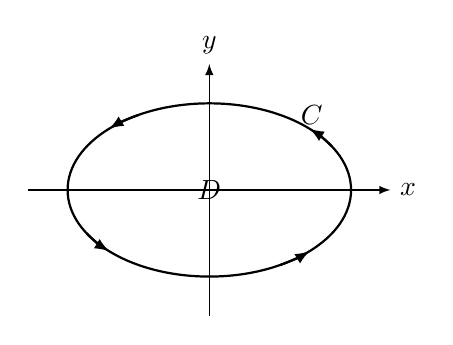
\begin{tikzpicture}[scale=1, >=latex]
			\draw[->] (-2.3,0) -- (2.3,0) node[right]{$x$};
			\draw[->] (0,-1.6) -- (0,1.6) node[above]{$y$};
			\draw[thick] (0,0) ellipse (1.8 and 1.1);
			\foreach \a in {30, 120, 210, 300} {
					\draw[->, thick] ({1.8*cos(\a)},{1.1*sin(\a)})
					arc[start angle=\a, end angle=\a+15, x radius=1.8, y radius=1.1];
				}
			\node at (1.3,0.95) {$C$};
			\node at (0,0) {$D$};
		\end{tikzpicture}
  \end{center}
\end{example}

\subsection{Curl and Divergence}

\begin{definition}{Curl}{curl}
  Let $\mathbf{F}\colon\R^3\to\R^3$, $\mathbf{F}(x,y,z)=
    \begin{bmatrix}
      P(x,y,z) \\Q(x,y,z)\\R(x,y,z)
    \end{bmatrix}
  $. The \emph{curl} of $\mathbf{F}$ is the vector field
  \[
    \operatorname{curl}\mathbf{F}
    = \left(\pd{R}{y}-\pd{Q}{z}\right)\hat{\mathbf{i}}
    + \left(\pd{P}{z}-\pd{R}{x}\right)\hat{\mathbf{j}}
    + \left(\pd{Q}{x}-\pd{P}{y}\right)\hat{\mathbf{k}}.
  \]
  As a map, $\operatorname{curl}\colon(\R^3\to\R^3)\to(\R^3\to\R^3)$.
\end{definition}

\begin{definition}{Divergence}{divergence}
  Let $\mathbf{F}\colon\R^3\to\R^3$ as above. The \emph{divergence} of $\mathbf{F}$ is the scalar field
  \[
    \operatorname{div}\mathbf{F}
    = \pd{P}{x} + \pd{Q}{y} + \pd{R}{z}.
  \]
  As a map, $\operatorname{div}\colon(\R^3\to\R^3)\to\R$.
\end{definition}

\textbf{Memorization via $\nabla$.} Let
\[
  \nabla =
  \begin{bmatrix}
    \partial/\partial x \\\partial/\partial y\\\partial/\partial z
  \end{bmatrix}
  .
\]
Then
\[
  \operatorname{curl}\mathbf{F} = \nabla\times\mathbf{F}
  = \det
  \begin{bmatrix}
    \hat{\mathbf{i}}    & \hat{\mathbf{j}}    & \hat{\mathbf{k}}    \\
    \partial/\partial x & \partial/\partial y & \partial/\partial z \\
    P                   & Q                   & R
  \end{bmatrix}
  \quad\text{(strictly 3D)},
  \qquad
  \operatorname{div}\mathbf{F} = \nabla\cdot\mathbf{F}.
\]

\textbf{Geometric meaning.} The curl measures local rotation of $\mathbf{F}$:

\begin{center}
  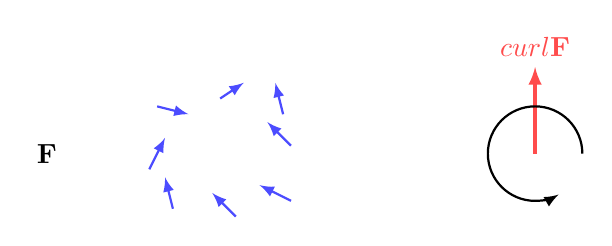
\begin{tikzpicture}[scale=1, >=latex]
		\foreach \x/\y/\dx/\dy in {
				-0.8/0.6/0.4/-0.1, 0/0.7/0.3/0.2, 0.8/0.5/-0.1/0.4,
				-0.9/-0.2/0.2/0.4, 0.9/0.1/-0.3/0.3,
				-0.6/-0.7/-0.1/0.4, 0.2/-0.8/-0.3/0.3, 0.9/-0.6/-0.4/0.2
			} {
				\draw[->, thick, blue!70] (\x,\y) -- ++(\dx,\dy);
			}
		\node at (-2.2,0) {$\mathbf{F}$};

		\begin{scope}[xshift=4cm]
			\draw[->, very thick, red!70] (0,0) -- (0,1.1) node[above]{$\operatorname{curl}\mathbf{F}$};
			\draw[->, thick] (0.6,0) arc[start angle=0, end angle=300, radius=0.6];
		\end{scope}
	\end{tikzpicture}
\end{center}

\begin{example}
  $\operatorname{div}\mathbf{F}=0$ corresponds to an incompressible flow velocity field.
\end{example}

\begin{theorem}{Curl of a Gradient}{curl-grad-zero}
  For a scalar field $f\colon\R^3\to\R$ with continuous second partials,
  \[
    \operatorname{curl}(\nabla f) = \mathbf{0}.
  \]
\end{theorem}

\begin{proof}
  \[
    \operatorname{curl}(\nabla f)
    =
    \begin{bmatrix}
      f_{yz} - f_{zy} \\
      f_{zx} - f_{xz} \\
      f_{xy} - f_{yx}
    \end{bmatrix}
    = \mathbf{0}
  \]
  by Clairaut's theorem on equality of mixed partials.
\end{proof}

\begin{remark}
  Equivalently, for any loop $C$, $\oint_C \nabla f\cdot\dd{\mathbf{r}}=0$ (FTLI).
\end{remark}

\begin{theorem}{Zero Curl Implies Conservative}{zero-curl-conservative}
  Let $\mathbf{F}$ be a vector field defined on all of $\R^3$ (or, more generally, on a simply connected open region in $\R^3$) whose component functions have continuous partial derivatives. Then
  \[
    \operatorname{curl}\mathbf{F}=\mathbf{0} \implies \mathbf{F} \text{ is conservative.}
  \]
\end{theorem}

\begin{remark}
  The simply-connected hypothesis is essential. The 3D embedding of the vortex
  $\mathbf{F}(x,y,z)=\ve{-y/(x^2+y^2),\,x/(x^2+y^2),\,0}$ on $\R^3\setminus\{z\text{-axis}\}$
  has $\operatorname{curl}\mathbf{F}=\mathbf{0}$ but is not conservative.
\end{remark}

\begin{theorem}{Divergence of a Curl}{div-curl-zero}
  For $\mathbf{F}\colon\R^3\to\R^3$ with continuous second partials,
  \[
    \operatorname{div}(\operatorname{curl}\mathbf{F}) = 0.
  \]
\end{theorem}

\begin{example}
  Find $\mathbf{G}\colon\R^3\to\R^3$ such that
  \[
    \operatorname{curl}\mathbf{G}
    =
    \begin{bmatrix}
      xz \\xy\\y\cos z
    \end{bmatrix}
    .
  \]
  By Theorem~\ref{thm:div-curl-zero}, $\operatorname{div}(\operatorname{curl}\mathbf{G})=0$. However,
  \[
    \pd{}{x}(xz) + \pd{}{y}(xy) + \pd{}{z}(y\cos z)
    = z + x - y\sin z
    \neq 0.
  \]
  Therefore $\mathbf{G}$ does not exist.
\end{example}

\subsection{Parametric Surfaces and Areas}

\begin{definition}{Parametric Surface}{parametric-surface}
  A \emph{parametric surface} is a vector-valued function
  \[
    \mathbf{r}(u,v) =
    \begin{bmatrix}
      x(u,v) \\ y(u,v) \\ z(u,v)
    \end{bmatrix}
  \]
  defined over a region $D$ in the $uv$-plane. Its image $S = \mathbf{r}(D)\subseteq\R^3$ is the surface.
\end{definition}

\begin{center}
  \begin{tikzpicture}[scale=0.9, >=latex]
		\draw[->] (-0.3,0) -- (2.6,0) node[right]{$u$};
		\draw[->] (0,-0.3) -- (0,2.2) node[above]{$v$};
		\draw[thick] (1.3,1) .. controls (1.9,1.5) and (1.7,0.4) .. (1.1,0.5)
		.. controls (0.7,0.55) and (0.8,1.3) .. (1.3,1);
		\node at (1.3,1) {$D$};
		\draw[|->, thick] (2.9,1) -- (4.2,1) node[midway, above]{$\mathbf{r}$};
	\end{tikzpicture}
  \hspace{0.5cm}
  \tdplotsetmaincoords{70}{120}
  \begin{tikzpicture}[tdplot_main_coords, scale=0.9, >=latex]
		\draw[->] (0,0,0) -- (3,0,0) node[below]{$x$};
		\draw[->] (0,0,0) -- (0,3,0) node[right]{$y$};
		\draw[->] (0,0,0) -- (0,0,3) node[above]{$z$};
		\draw[thick, blue!70, smooth, samples=40, domain=0:6.283, variable=\t]
		plot ({1.2 + 0.6*cos(\t r)}, {2.0 + 0.6*sin(\t r)}, {1.5 + 0.4*sin(2*\t r)});
		\node at (2.2,2.0,2.2) {$S$};
	\end{tikzpicture}
\end{center}

\begin{remark}
  Compare:
  \begin{align*}
    \text{curve in 3D:}   & \quad \mathbf{r}\colon\R\to\R^3   \\
    \text{surface in 3D:} & \quad \mathbf{r}\colon\R^2\to\R^3
  \end{align*}
\end{remark}

\textbf{Grid curves.} Fixing one variable produces a curve on $S$. For $u=u_0$,
\[
  \mathbf{r}(u_0,v) = \ve{x(u_0,v),\,y(u_0,v),\,z(u_0,v)}
\]
traces a curve on $S$ as $v$ varies, and vice versa for $v=v_0$.

\begin{example}[Cylinder]
  $\mathbf{r}(u,v) = \ve{2\cos u,\,v,\,2\sin u}$ parametrizes a cylinder of radius $2$ along the $y$-axis.

  \textbf{Fix $v=v_0$:}
  \[
    \mathbf{r}(u) = \ve{2\cos u,\,v_0,\,2\sin u}
  \]
  is a circle of radius $2$ centered at $\ve{0,v_0,0}$ in the plane $y=v_0$.

  \textbf{Fix $u=u_0$:}
  \[
    \mathbf{r}(v) = \ve{2\cos u_0,\,v,\,2\sin u_0}
  \]
  is a straight line parallel to the $y$-axis.

  \begin{center}
    \tdplotsetmaincoords{70}{120}
    \begin{tikzpicture}[tdplot_main_coords, scale=0.9, >=latex]
			\draw[->] (0,0,0) -- (3,0,0) node[below]{$x$};
			\draw[->] (0,0,0) -- (0,3.5,0) node[right]{$y$};
			\draw[->] (0,0,0) -- (0,0,3) node[above]{$z$};
			% cylinder body
			\draw[thick, blue!70] (2,0,0) -- (2,3,0);
			\draw[thick, blue!70] (-2,0,0) -- (-2,3,0);
			\draw[thick, blue!70] (0,0,2) -- (0,3,2);
			\draw[thick, blue!70] (0,0,-2) -- (0,3,-2);
			% circles at y=0, y=1.5, y=3
			\foreach \y in {0, 1.5, 3} {
					\draw[thick, red!70] plot[domain=0:360, samples=40, smooth]
					({2*cos(\x)}, \y, {2*sin(\x)});
				}
			\node[right] at (2.2,1.5,0) {\small circle, $r=2$};
		\end{tikzpicture}
    \hspace{0.8cm}
    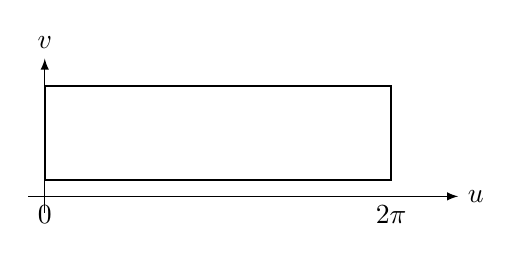
\begin{tikzpicture}[scale=0.7, >=latex]
			\draw[->] (-0.3,0) -- (7.5,0) node[right]{$u$};
			\draw[->] (0,-0.3) -- (0,2.5) node[above]{$v$};
			\draw[thick] (0,0.3) rectangle (6.2832,2);
			\node[below] at (0,0) {$0$};
			\node[below] at (6.2832,0) {$2\pi$};
		\end{tikzpicture}
  \end{center}
\end{example}

\begin{example}[Coiled tube]
  \[
    \mathbf{r}(u,v) =
    \begin{bmatrix}
      (2+\sin v)\cos u \\
      (2+\sin v)\sin u \\
      u + \cos v
    \end{bmatrix}
    =
    \underbrace{
      \begin{bmatrix}
        2\cos u \\ 2\sin u \\ u
      \end{bmatrix}
    }_{\text{helix coil}}
    +
    \underbrace{
      \begin{bmatrix}
        \sin v \cos u \\ \sin v \sin u \\ \cos v
      \end{bmatrix}
    }_{\text{circle of radius }1}
  \]
  Let $\hat{\mathbf{w}}(u) = \ve{\cos u,\,\sin u,\,0}$. Then the second term is
  \[
    \sin v\,\hat{\mathbf{w}} + \cos v\,\hat{\mathbf{k}},
  \]
  a unit circle in the plane spanned by $\hat{\mathbf{w}}$ and $\hat{\mathbf{k}}$. The surface is a tube of radius $1$ wound around the helix of radius $2$ ascending along the $z$-axis.

  \begin{center}
    \tdplotsetmaincoords{75}{110}
    \begin{tikzpicture}[tdplot_main_coords, scale=0.85, >=latex]
			\draw[->] (0,0,0) -- (3.5,0,0) node[below]{$x$};
			\draw[->] (0,0,0) -- (0,3.5,0) node[right]{$y$};
			\draw[->] (0,0,0) -- (0,0,7) node[above]{$z$};
			% central helix
			\draw[thick, gray!50, domain=0:18.85, samples=120, smooth, variable=\t]
			plot ({2*cos(\t r)}, {2*sin(\t r)}, {\t*0.3});
			% tube cross sections (circles) at sample u values
			\foreach \u in {0, 0.8, 1.6, 2.4, 3.2, 4.0, 4.8, 5.6, 6.4, 7.2, 8.0, 8.8, 9.6, 10.4, 11.2, 12.0, 12.8, 13.6, 14.4, 15.2, 16.0, 16.8} {
					\draw[thick, blue!60, domain=0:360, samples=20, smooth, variable=\v]
					plot ({(2+sin(\v))*cos(\u r)}, {(2+sin(\v))*sin(\u r)}, {\u*0.3 + cos(\v)});
				}
		\end{tikzpicture}
  \end{center}
\end{example}
